\documentclass[10pt]{article}
\usepackage{graphicx}
\usepackage{amssymb}
\usepackage{epstopdf}
\usepackage{tikz}
\usepackage{float}
\usepackage{enumitem}
\usepackage{multicol,multirow}
\DeclareGraphicsRule{.tif}{png}{.png}{`convert #1 `dirname #1`/`basename #1 .tif`.png}
\renewcommand{\tablename}{Tabla} 
\renewcommand{\figurename}{Figura} 
\newcommand*\circled[1]{\tikz[baseline=(char.base)]{\node[shape=circle,blue,draw,inner sep=1pt] (char) {#1};}}

% For a visual definition of these parameters, see
\textwidth = 6.5 in
\textheight = 9 in
\oddsidemargin = 0.0 in
\evensidemargin = 0.0 in
\topmargin = 0.0 in             
\headheight = 0.0 in            
\headsep = 0.0 in
            
\parskip = 0.2in                % vertical space between paragraphs
% Delete the % in the following line if you don't want to have the first line of every paragraph indented
%\parindent = 0.0in

\begin{document}
\begin{center}
    {\Large Prueba Especial, Programaci\'on II} \\
    \emph{\small Prof. Rodrigo Olivares} \\
    \emph{\scriptsize Julio 18, 2017}
\end{center}
\vspace*{-35pt}
\begin{center}
    \rule{1\textwidth}{.3pt}
\end{center}
\vspace*{-42pt}
\begin{center}
    \rule{1\textwidth}{2pt}
\end{center}

\vspace*{-15pt}
\textbf{Instrucciones}:
\vspace*{-15pt}

\begin{itemize}
    \item[-] El puntaje m\'aximo de la prueba especial es 100\%, siendo el 60\% el m\'inimo requerido para aprobar.
    \item[-] La prueba especial es \underline{\textbf{individual}}. Cualquier intento de copia, ser\'a sancionado con nota \textbf{1,0}.
\end{itemize}
\vspace*{-20pt}

\begin{enumerate}
    \item \emph{100pts.} Desarrolle el juego ``Advina la palabra'' bajo una aplicaci\'on JAVA, con Interfaz Gr\'afica de Usuario. La idea principal es tomar desde un archivo de texto, una palabra o frase al azar y ocultarla al jugador. El jugador intentar\'a adivinar la o las palabras, ingresando por teclado las letras que considere que son parte de la ella. El sistema ir\'a mostrando las letras que el usuario ingres\'o y que son parte de la palabra, incluso si se repiten en ella. No existe l\'imite de tiempo o de intentos, pero si se debe informar cu\'antas fueron las oportunidades que el usuario requiri\'o para completar el juego.

    \begin{itemize}
        \item \textbf{Reglas}
        \begin{itemize}
            \item El jugador s\'olo debe ingresar una letra por intento y presionar el bot\'on ``Jugar''.
            \item Al momento de presionar el bot\'on ``Jugar'' el sistema debe validar que el jugador halla ingresado la letra en el campo de texto.
            \item Se debe mostrar la palabra oculta, y cada vez que el usuario adivine una letra, se debe mostrar en la palabra semi-completada. Si la letra est\'a repetida en la palabra, se deben mostrar todas las coincidencias.
            \item No se deben consierar intentos, las letras repetidas ingresads por el usuario. Se debe informar al jugador que esa letra ya fue ingresda.
            \item Al advinar la palabra, se debe mostrar la cantidad de intentos v\'alidos que tard\'o el jugador en terminar el juego y se debe almacenar en un archivo e texto.
        \end{itemize} 
        \item \textbf{Restricciones}
        \begin{itemize}
            \item Paradigma de Orientaci\'on a Objetos.
        \end{itemize} 
            \end{itemize}    
        \item[] Una estructura gr\'afica b\'asica, puede ser la siguiente:
        
        \begin{figure}[H]
        \begin{center}
            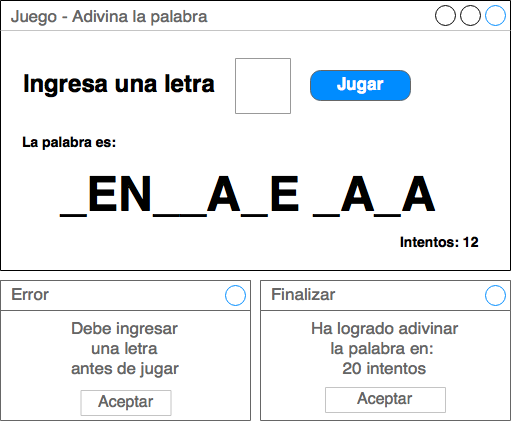
\includegraphics[scale=.5]{ejemplo.png}
        \end{center}
        \end{figure}
    
   
    
    
\end{enumerate}

\end{document} 
